\documentclass[11pt,]{article}
\usepackage[left=1in,top=1in,right=1in,bottom=1in]{geometry}
\newcommand*{\authorfont}{\fontfamily{phv}\selectfont}
\usepackage[]{mathpazo}


  \usepackage[T1]{fontenc}
  \usepackage[utf8]{inputenc}



\usepackage{abstract}
\renewcommand{\abstractname}{}    % clear the title
\renewcommand{\absnamepos}{empty} % originally center

\renewenvironment{abstract}
 {{%
    \setlength{\leftmargin}{0mm}
    \setlength{\rightmargin}{\leftmargin}%
  }%
  \relax}
 {\endlist}

\makeatletter
\def\@maketitle{%
  \newpage
%  \null
%  \vskip 2em%
%  \begin{center}%
  \let \footnote \thanks
    {\fontsize{18}{20}\selectfont\raggedright  \setlength{\parindent}{0pt} \@title \par}%
}
%\fi
\makeatother




\setcounter{secnumdepth}{3}


\usepackage{graphicx,grffile}
\makeatletter
\def\maxwidth{\ifdim\Gin@nat@width>\linewidth\linewidth\else\Gin@nat@width\fi}
\def\maxheight{\ifdim\Gin@nat@height>\textheight\textheight\else\Gin@nat@height\fi}
\makeatother
% Scale images if necessary, so that they will not overflow the page
% margins by default, and it is still possible to overwrite the defaults
% using explicit options in \includegraphics[width, height, ...]{}
\setkeys{Gin}{width=\maxwidth,height=\maxheight,keepaspectratio}

\title{Título\\
Subtítulo\\
Subtítulo  }



\author{\Large Ana Hilda Valera Arias\vspace{0.05in} \newline\normalsize\emph{Estudiante, Universidad Autónoma de Santo Domingo (UASD)}  }


\date{}

\usepackage{titlesec}

\titleformat*{\section}{\normalsize\bfseries}
\titleformat*{\subsection}{\normalsize\itshape}
\titleformat*{\subsubsection}{\normalsize\itshape}
\titleformat*{\paragraph}{\normalsize\itshape}
\titleformat*{\subparagraph}{\normalsize\itshape}

\titlespacing{\section}
{0pt}{36pt}{0pt}
\titlespacing{\subsection}
{0pt}{36pt}{0pt}
\titlespacing{\subsubsection}
{0pt}{36pt}{0pt}





\newtheorem{hypothesis}{Hypothesis}
\usepackage{setspace}

\makeatletter
\@ifpackageloaded{hyperref}{}{%
\ifxetex
  \PassOptionsToPackage{hyphens}{url}\usepackage[setpagesize=false, % page size defined by xetex
              unicode=false, % unicode breaks when used with xetex
              xetex]{hyperref}
\else
  \PassOptionsToPackage{hyphens}{url}\usepackage[unicode=true]{hyperref}
\fi
}

\@ifpackageloaded{color}{
    \PassOptionsToPackage{usenames,dvipsnames}{color}
}{%
    \usepackage[usenames,dvipsnames]{color}
}
\makeatother
\hypersetup{breaklinks=true,
            bookmarks=true,
            pdfauthor={Ana Hilda Valera Arias (Estudiante, Universidad Autónoma de Santo Domingo (UASD))},
             pdfkeywords = {Género, Planta},  
            pdftitle={Título\\
Subtítulo\\
Subtítulo},
            colorlinks=true,
            citecolor=blue,
            urlcolor=blue,
            linkcolor=magenta,
            pdfborder={0 0 0}}
\urlstyle{same}  % don't use monospace font for urls

% set default figure placement to htbp
\makeatletter
\def\fps@figure{htbp}
\makeatother

\usepackage{pdflscape} \newcommand{\blandscape}{\begin{landscape}}
\newcommand{\elandscape}{\end{landscape}}


% add tightlist ----------
\providecommand{\tightlist}{%
\setlength{\itemsep}{0pt}\setlength{\parskip}{0pt}}

\begin{document}
	
% \pagenumbering{arabic}% resets `page` counter to 1 
%
% \maketitle

{% \usefont{T1}{pnc}{m}{n}
\setlength{\parindent}{0pt}
\thispagestyle{plain}
{\fontsize{18}{20}\selectfont\raggedright 
\maketitle  % title \par  

}

{
   \vskip 13.5pt\relax \normalsize\fontsize{11}{12} 
\textbf{\authorfont Ana Hilda Valera Arias} \hskip 15pt \emph{\small Estudiante, Universidad Autónoma de Santo Domingo (UASD)}   

}

}








\begin{abstract}

    \hbox{\vrule height .2pt width 39.14pc}

    \vskip 8.5pt % \small 

\noindent Resumen del manuscrito


\vskip 8.5pt \noindent \emph{Keywords}: Género, Planta \par

    \hbox{\vrule height .2pt width 39.14pc}



\end{abstract}


\vskip 6.5pt


\noindent  \section{Introducción}\label{introducciuxf3n}

La vegetación terrestre está constituida por un conjunto de plantas
pertenecientes a una familia en específico y esta a su vez se subdividen
en géneros y especies para identificarse dentro de su clase. Por
consiguiente no sería la excepción de la malvaceae, poseen 243 genéros y
más de 4,300 especies, sus flores son hermafroditas, pocas veces
unisexuales, solitarias o fasciculadas en las axilas de las hojas o
agrupadas en inflorescencia tal como la describen los siguientes autores
(Marín, Hilario, \& Andino, n.d.) y (Bayer, 2003).

Dentro de los géneros a encontrar en la familia malvaceae están el
abutilon constituido por arbustos, subarbustos y hierbas bienales con
pelo estrellados y tallos velloso, son carente del epicáliz conjunto de
apéndices que por lo regular tienen otros grupos de dicha familia, así
como de tener alrededor de 150 especie nativa en los trópicos y
subtrópicos de América, África, Asia y Australia, (Lorenzo-Cáceres,
2007). También, está el Hibiscus donde los segmentos del epicáliz estan
libres o unidos en la base, con estigmas alargados, semillas reniformes
y numerosas, (ORTIZ, 2010). Del mismo modo, se encuentra la althaea,
lavatera y la malva cada una contienen sus respectivas especies las
cuales pueden encontrarse en mayor o menor proporción en un espacio
determinado la cual dependerá de factores abioticos incidentes entre
ellos, lo que implicaría la necesidad de utilizar tecnicas y análisis
numerológicos para conocer su asocianción.

La implementación de análisis numéricos en las investigaciones
ecológicas permiten dar a conocer en terminos cuantificables la forma en
que se encuentran asociadas y el tipo de patrón que presenta algunas
especies, es por ello la importancia de la estratificación y
zonificación del objeto de estudio en cuestión. De acuerdo con
(González, 2006) esto permite conjugar en un mismo grupo información de
aquellos organismos que pueden ser cuantificable junto con otros que son
reproductivos y de manera general con toda la vegetación.

Este estudio busca conocer cómo estan asociados los diferentes géneros y
especies de la familia malvaceae y si las variables ambientales
existente en la zona influyen en dicha asociación. También, analizar
como estan organizados los grupos y qué patrón presentan en caso de que
existiese, así, como establecer los indicadores ambientales que
interfieren. De igual manera, examinar en qué volumen se encuentran
representadas cada una y distiguir las especies alpha y beta, además, de
construir modelos de distribución espacial para idenficarla. En tal
sentido, esta investigación constribuirá al conocimiento de la dinámica
ecológica espacial que envuelven las plantas pertenecientes a la familia
malvaceae en la isla Barro Colorado que en lo adelante será llamado BCI
y con la misma gestionar estrategias para el cuidado y conservación de
estas.

\ldots

\section{Metodología}\label{metodologuxeda}

\subsection{Área de estudio}\label{uxe1rea-de-estudio}

La isla Barro Colorado se encuentra ubicada en el canal de Pánama en las
proximidades del lago Gatún, de acuerdo con (Pérez et al., 2005) esta se
formó cuando se construyó dicho canal embalsando las aguas del río
Chagres, se localiza entre las coordenadas geográficas 9 grados con 09
minutos al Norte y 79 grados con 51 minutos al Oeste y cubre una
extensión de tierra de 1,500 hectáreas (ver figura \ref{mapa}). El clima
es de bosque tropical, la temperatura promedio es de 27 grados
centígrados, con temporadas lluviosas durante los meses mayo-diciembre y
secas desde mediados de diciembre hasta abril, las tormentas convectivas
son prevenidas por los vientos alisios dictando así las estaciones del
año, (Sugasti, Eng, \& Pinzón, 2018).

\begin{figure}
\centering
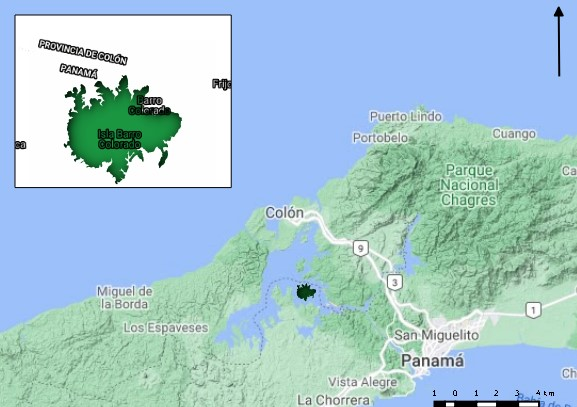
\includegraphics{mapa_barro_colorado.jpeg}
\caption{Ubicación de la isla Barro Colorado\label{mapa}}
\end{figure}

\ldots

\section{Resultados}\label{resultados}

\ldots

\section{Discusión}\label{discusiuxf3n}

\section{Agradecimientos}\label{agradecimientos}

\section{Información de soporte}\label{informaciuxf3n-de-soporte}

\ldots

\section{\texorpdfstring{\emph{Script}
reproducible}{Script reproducible}}\label{script-reproducible}

\ldots

\section*{Referencias}\label{referencias}
\addcontentsline{toc}{section}{Referencias}

\hypertarget{refs}{}
\hypertarget{ref-bayer2003malvaceae}{}
Bayer, K., Clemens y Kubitzki. (2003). Malvaceae. In Springer (Ed.),
\emph{Plantas con flores ~textperiodcentered dicotiledóneas}.

\hypertarget{ref-gonzalez2006ecologia}{}
González, A. R. (2006). \emph{Ecología: Métodos de muestreo y análisis
de poblaciones y comunidades}. Pontificia Universidad Javeriana.

\hypertarget{ref-de2007especies}{}
Lorenzo-Cáceres, J. M. S. de. (2007). Las especies del género abutilon
mill.(Malvaceae) cultivadas en españa. \emph{PARJAP: Boletín de La
Asociación Española de Parques Y Jardines}, (45), 45--49.

\hypertarget{ref-marinanalisis}{}
Marín, J. Z., Hilario, R. F., \& Andino, O. O. (n.d.). \emph{Análisis
filogenético de la familia malvaceae}.

\hypertarget{ref-ortizclaves}{}
ORTIZ, D. G. (2010). \emph{Claves para los taxones y cultones del género
hibiscus l.(Malvaceae) cultivados y comercializados en la comunidad
valenciana (e españa)}.

\hypertarget{ref-perez2005metodologia}{}
Pérez, R., Aguilar, S., Condit, R., Foster, R., Hubbell, S., \& Lao, S.
(2005). Metodologia empleada en los censos de la parcela de 50 hectareas
de la isla de barro colorado, panamá. \emph{Centro de Ciencias
Forestales Del Tropico (CTFS) Y Instituto Smithsonian de Investigaciones
Tropicales (STRI)}, 1--24.

\hypertarget{ref-sugastimedicion}{}
Sugasti, L., Eng, B., \& Pinzón, R. (2018). \emph{Medición continúa de
flujo de co2 ensuelo en una parcela de bosque tropical en isla barro
colorado, canal de panamá.}




\newpage
\singlespacing 
\end{document}
